\documentclass[10pt,a4paper]{article}
\usepackage[latin1]{inputenc}
\usepackage{amsmath}
\usepackage{microtype}
\usepackage[none]{hyphenat}
\usepackage{verbatim}
\usepackage{amsfonts}
\usepackage{amssymb}
\usepackage{enumitem}
\renewcommand{\familydefault}{\sfdefault}
\usepackage{mathpazo}
\renewcommand{\rmdefault}{put}
\usepackage{enumitem}
\usepackage[dvipsnames,svgnames]{xcolor}
\usepackage{tkz-euclide}
\usetkzobj{all}
\usepackage{graphicx}
\usepackage{tikz} 	
\usepackage{adjustbox}
\usepackage{multicol}
\usepackage{lipsum}
\usepackage[left=0.1cm,right=0.7cm,top=0.2cm,bottom=1.5cm]{geometry}
\usepackage{cancel} \usepackage{xcolor}
\usepackage{tcolorbox}
\usetikzlibrary{decorations.pathmorphing,patterns}
\usetikzlibrary{decorations.pathreplacing,calc}
 \newcommand\coret[2][red]{\renewcommand\CancelColor{\color{#1}}\cancel{#2}}

%%_------= solusi


% Set this =0 to hide, =1 to show

% Set this =0 to hide, =1 to show
\newtcolorbox{mybox}[1][] { colframe = blue!10, colback = blue!3,boxsep=0pt,left=0.2em, coltitle = blue!20!black, title = \textbf{jawab}, #1, } 


\def\showanswers{1}
\newcommand{\hide}[1]{\ifnum\showanswers=1
%
\begin{mybox}
 #1
\end{mybox}
%
\vspace{\baselineskip}\fi\ifnum\showanswers=0\vspace{2\baselineskip} \hspace{2cm}\fi}



\newcommand*\cicled[1]{\tikz[baseline=(char.base)]{\node[white, shape=circle, fill=red!80,draw,inner sep=0.5pt](char){#1};}}

\newcommand*\lingkaran[1]{\tikz[baseline=(char.base)]{\node[red, shape=circle,draw,inner sep=0.5pt](char){#1};}\stepcounter{enumii}}

\newcommand*\silang[1]{\tikz[baseline=(char.base)]{
\draw[red,thick](-0.2,-0.20)--(0.2,0.2);
\draw[red,thick](-0.2,0.20)--(0.2,-0.2);
\node[black](char){#1};
}}


\newcommand*\centang[1]{\tikz[baseline=(char.base)]{
\draw[red, very thick](-0.2,0.1)--(-0.1,0)--(0.2,0.3);
\node(char){#1};
}}

\newcommand*\merah[1]{
\textcolor{red}{#1}}
\newcommand*\pilgan[1]{
\begin{enumerate}[label=\Alph*., itemsep=0pt,topsep=0pt,leftmargin=*] #1 
\end{enumerate}}
\newcommand*\pernyataan[1]{
\begin{enumerate}[label=(\arabic*), itemsep=0pt,topsep=0pt,leftmargin=*] #1 
\end{enumerate}}



\begin{document}

\setlength{\abovedisplayskip}{0pt}
\setlength{\belowdisplayskip}{3pt}
\setlength{\abovedisplayshortskip}{0pt}
\setlength{\belowdisplayshortskip}{3pt}
%-----------------------------------------------

 \centering
  \renewcommand{\arraystretch}{2}
  \begin{tabular}{  |>{\centering\arraybackslash}m{4cm}|%
                    >{\centering\arraybackslash}m{11cm}|%
                    >{\centering\arraybackslash}m{4cm}|%
  }
    \hline
    \vspace{0.15cm} 
    \tikz[baseline=(char.base)]{
\draw[green!80!black](-0.3,-0.2) rectangle (0.3,0.2);
\node[green](char){line};
} \small{ arifstwan} &       \textbf{Soal Modul Momentum } 
          &  bintangpelajar.com
  \\ \hline 
    
  \end{tabular}
\setlength{\columnsep}{0pt}
\vspace{0.15cm}

\begin{multicols*} {3} 
\newcommand{\tikzmark}[2]{\tikz[remember picture,baseline=(#1.base)]{\node[inner sep=0pt] (#1) {#2};}} 


\begin{enumerate}[itemsep=0mm]

%nomer 1
\item Manakah dari pernyataan berikut ini yang akan menghasilkan impuls
\pernyataan{
\item Sebuah bola ditendang murid 
\item Satelit mengelilingi bumi mengikuti orbit tetap
\item Seorang murid tersandung batu
\item Seekor ikan yang berenang dengan cepat
}
\pilgan{
\item 1,2, dan 3 
\item [\lingkaran{B.}]1 dan 3 
\item 2 dan 4
\item 4 saja
\item 1,2,3, dan 4
}
\hide{
impuls \\
$I=F.\Delta t= \Delta p = m (v_2-v_1)$
\pernyataan{
\item Sebuah bola ditendang murid
\centang{ } \merah{\small{bola setelah mendapat gaya $F$ pada selang waktu $\Delta t$, menimbulkan Impuls $I=F.t$}}
\item Satelit mengelilingi bumi  mengikuti orbit tetap \silang{ }\merah{\small{satelit bergerak dengan besar kecepatan yang sama, padahal impuls mensyaratkan perubahan kecepatan}}
\item Seorang murid tersandung batu \centang{ } \merah{\small{murid saat tersandung kemungkinan akan berhenti, jadi perubahan kecepatan dari v menjadi 0, maka terjadi impuls}}
\item Seekor ikan yang berenang dengan cepat
\silang{ }\merah{\small{ikan berenang dengan cepat tidak menunjukkan perubahan kecepatan, maupun momentum}}
}}

\item Di antara benda berikut ini yang akan mengalami gaya terbesar bila menumbuk tembok berhenti dalam selang waktu yg sama adalah . . . 
\pilgan{
\item benda bermassa 40 kg dengan kecepatan 25 m/s
\item benda bermassa 50 kg dengan kecepatan 15 m/s
\item benda bermassa 100 kg dengan kecepatan 10 m/s
\item [\lingkaran{D.}] benda bermassa 150 kg dengan kecepatan 7 m/s
\item benda bermassa 200 kg dengan kecepatan 5 m/s
}
\hide{
jika berhenti berarti kecepatan akhir=0, dan selang waktu sama\\
\begin{align*}
I&=F.\Delta t=m(v_2-v_1)\\
F&=\frac{m(0-v_1)}{\Delta t}=\frac{mv}{t}
\end{align*}
jadi $F$ sebanding dengan $m.v$\\
A. $m.v=40.50=2000$ \\
B. $m.v=50.15=750$\\
C. $m.v=100.10=1000$\\
D. $m.v=150.7=1050$ \centang { }\\
E. $m.v=200.5=1000$\\
}

\item Sebuah mobil bermassa 2.000kg sedang bergerak dengan kecepatan 72 km/jam. Momentum mobil tersebut adalah. . . . \\ 
\pilgan{
\item 20.000 kg m/s
\item 35.000 kg m/s
\item[\lingkaran{C.}]40.000 kg m/s
\item 92.000 kg m/s
\item 144.000 kg m/s
}
\hide{
$m$=2.000 kg, $v$=20 m/s 
\begin{align*}
p&=mv\\
p&=2000.20\\
p&=40000\text{kg m/s}
\end{align*}
}
%nomer 2
\item Sebuah truk bermassa 2.000 kg melaju dengan kecepatan 36 km/jam, kemudian menabrak sebuah pohon dan berhenti pada waktu 0,1 s. Gaya rata-rata pada truk tersebut selama berlangsungnya tabrakan adalah . . . 
\pilgan{
\item 200 N
\item 2.000 N
\item 20.000 N
\item [\lingkaran{D.}]200.000 N
\item 2.000.000 N
}

\hide{
diketahui : $v$=36km/jam = 10 m/s \\
$m$=20.000 kg, $v_2$=0 m/s, $\Delta t= 0$s 
ditanya :$F$
\begin{align*}
\Delta p &= I\\
m(v_2-v_1)&=F.t\\
2000(0-10)&=F.0,1\\
\frac{-200.000}{0,1}&=F\\
-200.000 \text{N} &=F
\end{align*}
artinya gaya yg bekerja pada truk 200.000 N berlawanan arah gerak truk
} 


\item Sebuah benda bergerak lurus di bawah pengaruh resultan gaya tetap. Selama 4s, momentum linear benda berubah dari 4 kgm/s menjadi 12 kgm/s dengan arah gerak akhir berlawanan dengan arah gerak mula-mula. Resultan gaya pada benda itu besarnya . . . 
\pilgan{
\item 2 N
\item [\lingkaran{B.}]4 N
\item 8 N
\item 10 N
\item 12 N
}
\hide{
diketahui : $p_1$= 4 kgm/s \\
$p_2$=-12 kgm/s (arah berlawanan)\\
$t$=4s\\
ditanya: $F$...?
\begin{align*}
\Delta p &= I\\
p_2 - p_1 &=F.t\\
-12 - 4 &= F. 4\\
\frac{-16}{4}&=F\\
-4 \text{N}&=F
\end{align*}
}

\item  Sebuah gaya 2 N bekerja pada sebuah benda. Jika diketahui bahwa perubahan momentum pada benda 120 kg m/s, berapa lama gaya tersebut beraksi?
\pilgan{
\item 50 s
\item [\lingkaran{B.}]60 s
\item 70 s
\item 80 s
\item 90 s
}
\hide{
perubahan momentum\\
 $\Delta p=I=F.\Delta t$\\
sehingga,
\begin{align*}
\Delta p& = F.\Delta t\\
\Delta t&= \frac{\Delta p}{F}=\frac{120}{2}=60s
\end{align*}
}

\item sebuah bola bermassa 0,25 kg bergerak dengan kelajuan 13 m/s. Berapakah gaya yang dibutuhkan untuk memukul bola dengan pemukul kayu agar berubah arah dengan kecepatan 19 m/s, jika waktu kontak pemukul dan bola adalah 0,01 s. . . .\\
\pilgan{
\item 150 N
\item 200 N
\item 250 N
\item 600 N
\item [\lingkaran{E.}]800 N
}
\hide{
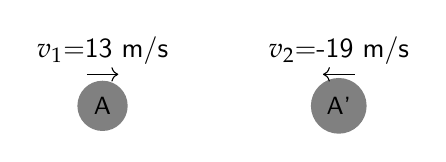
\begin{tikzpicture}
\node at (0,0) [fill=gray,circle]{\small{A}};
\draw[->] (-0.2,0.4) -- node [midway, above] {$v_1$=13 m/s}(0.2,0.4); 
\node at (3,0) [fill=gray,circle]{\small{A'}};
\draw[->] (3.2,0.4) -- node [midway, above] {$v_2$=-19 m/s}(2.8,0.4); 
\end{tikzpicture}
berdasarkan gambar tampak bahwa kecepatan akhir menjadi negatif (karena berubah arah), maka rumus Impuls- momentum berlaku:
\begin{align*}
I&=F.\Delta t\\
\Delta p&= F.\Delta t\\
m(v_2-v_1)&=F. \Delta t\\
\frac{0,25.(-19-13)}{0,01}&=F\\
F&=800 \text{N}
\end{align*}
}

\item Sebuah bola bermassa 0,2 kg dalam keadaan diam, kemudian dipukul sehingga meluncur dengan kecepatan 100 m/s dan pemukul menyentuh bola selama 0,1s. Besar gaya pemukul adalah . . . . \\
\pilgan{
\item 35 N
\item 50 N
\item 100 N
\item 150 N
\item [\lingkaran{E.}]200 N
}
\hide{
$v_1=0$, $v_2=100$ m/s.
\begin{align*}
I&=F.\Delta t\\
\Delta p&= F.\Delta t\\
m(v_2-v_1)&=F. \Delta t\\
\frac{0,2.(-100-0)}{0,1}&=F\\
F&=200 \text{N}
\end{align*}
}
\item Sebuah bola pada permainan softball bermassa 0,15 kg dilempar horisontal ke kanan dengan kelajuan 20 m/s. Setelah dipukul, bola bergerak dengan kelajuan 20 m/s ke kiri. Impuls yang diberikan kayu pemukul terhadap bola adalah . . . 
\pilgan{
\item 2 Ns
\item 4 Ns
\item [\lingkaran{C.}]6 Ns
\item 8 Ns
\item 10 Ns
}
\hide{
$m$=0,15 kg\\
$v_1=20 \text{m/s}$,  $v_2=-20$ m/s (kiri)\\
Impuls  $I$=...?
\begin{align*}
I&=F.\Delta t = \Delta p\\
I&=m (v_2-v_1)=0,15(-20-20)\\
I&=6\text{ N}
\end{align*}
}


\item Gambar di bawah ini menunjukkan resultan gaya yang bekerja pada suatu benda terhadap waktu. Besar perubahan momentum benda setelah 15 s adalah . . . .\\
\begin{tikzpicture}[scale=0.3]
\draw [<->](0,12)node [above left] {F}--(0,0)--(17,0)node [below right] {t};
\foreach \x  in {5,10,15}
{ \node at (\x,0)[below,scale=1.2]{\x}; 
} 
\draw(0,10) node [left,scale=1.2] {10}--(5,10)--(15,0);
\draw[dashed](5,10)--(5,0)--(10,0)--(10,5)--(0,5);
\node at (0,5) [left,scale=1.2] {5};
\end{tikzpicture}
\pilgan{
\item 50 Ns
\item [\lingkaran{B.}]100 Ns
\item 150 Ns
\item 200 Ns
\item 250 Ns
} 
\hide{
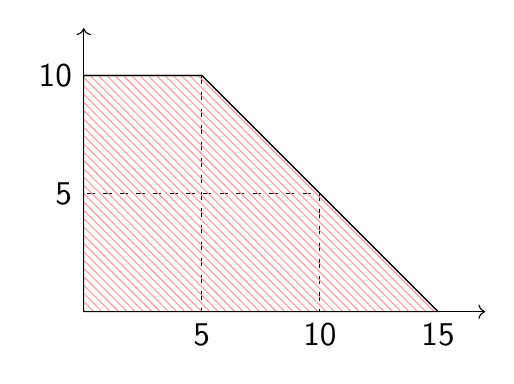
\begin{tikzpicture}[scale=0.3]
\draw [<->](0,12)--(0,0)--(17,0);
\foreach \x  in {5,10,15}
{ \node at (\x,0)[below,scale=1.2]{\x}; 
} 
\draw(0,10) node [left,scale=1.2] {10}--(5,10)--(15,0);
\draw[dashed](5,10)--(5,0)--(10,0)--(10,5)--(0,5);
\draw[pattern=north west lines,pattern color=red!40] (0,10)--(5,10)--(15,0)--(0,0)--cycle;
\node at (0,5) [left,scale=1.2] {5};
\end{tikzpicture}

Besar perubahan momentum $\Delta p= I=F.\Delta t$\\
$\Delta p=\int F(t) dt$ = Luasan grafik\\
$\Delta p=\text{luas trapesium}$\\
$\Delta p=\frac{5+15}{2}{10}$\\
$\Delta p=100$ Ns
}


\item Perhatikan grafik gaya ($F$) vs waktu ($t$) di bawah ini!\\
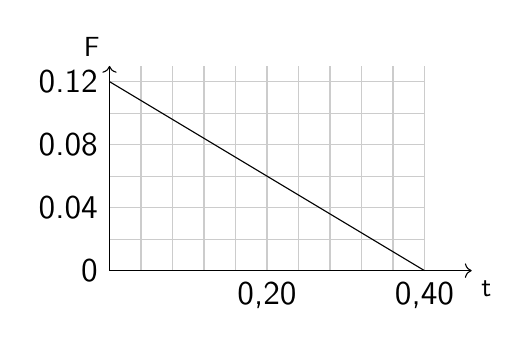
\begin{tikzpicture}[scale=0.2]

\draw [gray!40] (0,0) grid [step=2cm] (20,13);
\draw [<->](0,13)node [above left] {F}--(0,0)--(23,0)node [below right] {t};
\foreach \l / \y  in {0/0,0.04/4,0.08/8,0.12/12}
{ \node at (0,\y)[left,scale=1.2]{\l}; 
}
\node at (10,0) [below, scale=1.2] {0,20}; 
\node at (20,0) [below, scale=1.2] {0,40}; 

\draw(0,12) --(20,0);
\end{tikzpicture}
Besar impuls adalah . . . . \\
\pilgan{
\item [\lingkaran{A.}]0,024 Ns
\item 0,011 Ns
\item 0,005 Ns
\item 0.0101 Ns
\item 0,204 Ns
}

\hide{
Besar Impuls $I=F.\Delta t$\\
$I=\int F(t) dt$ = Luasan grafik\\
$I=\text{luas segitiga}$\\
$I=\frac{1}{2}0,4.0,12$\\
$I=0,024$ Ns
}

\item Dua benda titik bermassa $m_1$ = 5kg dan $m_2$ = 6 kg terletak berdekatan di bidang datar licin. Sistem ini mendapat impuls gaya hingga kedua benda bergerak masing-masing dengan laju $v_1$ = 1 m/s dan $v_2$ = 2 m/s dengan arah saling tegak lurus. Besarnya impuls gaya yg bekerja pada sistem ini adalah. . . .\\
\pilgan{
\item [\lingkaran{A.}]13,0 Ns
\item 15,0 Ns
\item 16,0 Ns
\item 17,0 Ns
\item 18,0 Ns
}
\hide{
\begin{align*}
I&=\Delta p\\
I&=\sqrt{\Delta p_x^2+\Delta p_y^2}\\
I&=\sqrt{(m_1.\Delta v_1)^2+(m_2.\Delta v_2)^2}\\
I&=\sqrt{(5.1)^2+(6.2)^2}=13 Ns
\end{align*}
}

\item Sebuah bola A yang mempunyai momentum $p$ bertumbukam dengan bola B sehingga setelah tumbukam momentum bola A tersebut menjadi 3p. Perubahan momentum bola B adalah . . . .\\
\pilgan{
\item -3$p$
\item [\lingkaran{B.}]-2$p$
\item $p$
\item 2$p$
\item 4$p$
}
%
\hide{
\begin{align*}
\Sigma p_1&=\Sigma p_2\\
p_A+p_B&=p_A'+p_B'\\
p+p_B&=3p+p_B'\\
-2p&=p_B'-p_B\\
-2p&=\Delta p_B
\end{align*}
}

\item Sebuah benda bergerak dengan momentum $p$. Tiba-tiba benda itu pecah menjadi dua bagian yang besar momentumnya masing-masing $p_1$ dan $p_2$ dalam arah yang tegak lurus. Momentum benda dapat dinyatakan sebagai. . . . \\
\pilgan{
\item $p=p_1+p_2$
\item $p=p_1-p_2$
\item $p=p_2-p_1$
\item [\lingkaran{D.}]$p=({p_1}^2+{p_2}^2)^{\frac{1}{2}}$
\item $p=({p_1}^2+{p_2}^2)$
}
\hide{
tegak lurus. Kita anggap benda 1 ke arah $x$ dan benda 2 ke arah $y$ maka jumlah momentumnya \\
$p=\sqrt{p_x^2+p_y^2}$\\
$p=({p_1}^2+{p_2}^2)^{\frac{1}{2}}$
}

\item Sebuah benda bermassa 2,5 kg diletakkan mendatar di atas sebuah meja licin dari keadaan diam oleh sebuah gaya mendatar $F$. Gaya $F$ tersebut berubah terhadap waktu menurut $F=80+5t$, dengan $t$ dalam s dan $F$ dalam N. Pada saat $t=2$ s, momentum benda tersebut adalah . . . \\
\pilgan{
\item 85 kg m/s
\item 125 kg m/s
\item 150 kg m/s
\item [\lingkaran{D.}]170 kg m/s
\item 340 kg m/s
}
\hide{
keadaan awal diam, maka momentum awal = 0
\begin{align*}
I&=F.\Delta t\\
p_2-p_1&=\int_0^2 (80+5t) dt\\
p_2 &=80t+\frac{5t^2}{2}\\
p_2&=170
\end{align*}
}


\item Sebuah bola bermassa 100 g dijatuhkan dari ketinggian $h_1$=1,8 m di atas lantai, bola memantul setinggi $h_2$=1,25 m. Hitung impuls yang dikerjakan lantai pada bola?
\pilgan{
\item 0,11 Nm
\item 0,11 Nm
\item [\lingkaran{C.}]1,10 Nm
\item 11 Nm
\item 110 Nm
}

\hide{
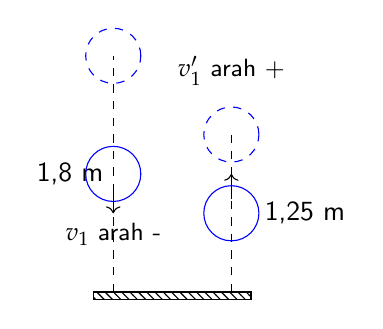
\begin{tikzpicture}[scale=0.5]
\draw[pattern=north west lines](0,-0.2) rectangle (4,0);
\draw[dashed](0.5,0)-- node [midway, left]{1,8 m}(0.5,6);
\draw[dashed](3.5,0)-- node [midway, right,xshift=0.3cm]{1,25 m}(3.5,4);
\foreach \x/\y in {0.5/3,3.5/2}{
\node at(\x,\y) [circle,draw, blue, minimum size=0.7cm]{ };}
\foreach \x/\y in {0.5/6,3.5/4}{
\node at(\x,\y) [dashed, circle,draw, blue, minimum size=0.7cm]{ };}
\draw[->](0.5,2.65)--(0.5,2) node [below] {\small $v_1$ arah -};
\draw[->](3.5,2.35)--(3.5,3) node [above, yshift=1cm] {\small $v_1'$ arah +};
\end{tikzpicture}
}
\hide{
Kecepatan benda dari ketinggian tertentu atau mencapai ketinggian tertentu $v=\sqrt{2gh}$
\begin{align*}
I&=\Delta p\\
I&=m.(v_2-v_1)\\
I&=0,1.(\sqrt{2gh_2} - - \sqrt{2gh_1})\\
I&=0,1.(\sqrt{2.10.1,25} - - \sqrt{2.10.1,8})\\
I&=0,1.(\sqrt{25}+\sqrt{36})\\
I&=0,1.11=1,10 \text{ Ns}
\end{align*}
}


\item Sebuah benda bermassa 0,5 kg yang sedang bergerak dengan kecepatan 2 m/s ke timur menabrak benda lain yang bermassa 0,3 kg yang bergerak 4 m/s ke arah barat. Setelah tabrakan, benda 0,3 kg bergerak 2 m/s ke timur. Berapakah besar kecepatan benda 0,5 kg?
\pilgan{
\item [\lingkaran{A.}]1,6 m/s ke barat
\item 1,6 m/s ke timur
\item 0
\item 16 m/s ke barat
\item 16 m/s ke timur
}
\hide{
diketahui $m_A=0,5$ kg\\
\phantom{diketahui} $v_A$=2 m/s\\
\phantom{diketahui} $m_B$=0,3 kg\\
\phantom{diketahui} $v_B$=-4 m/s\\
\phantom{diketahui} $v_B'$=2 m/s\\
ditanya : $v_A'$= . . . . ?\\
\begin{align*}
\Sigma p &= \Sigma p'\\
m_A.v_A+m_B.v_B&=m_A.v_A'+m_B.v_B'\\
0,5.2+0,3(-4)&=0,5.v_A'+0,3.2\\
1,0-1,2&=0,5.v_A'+0,6\\
v_A&=-1,6 
\end{align*}
- artinya ke barat
}



\item Bola A dan B masing-masing massanya 20 kg dan 5 kg. Bola B diam ditumbuk bola A sehingga keduanya menyatu bergerak dengan kecepatan 2 m/s. Kecepatan bola A sebelum menumbuk adalah . . . . \\
\pilgan{
\item 1,5 m/s
\item 2,0 m/s
\item [\lingkaran{C.}]2,5 m/s
\item 4,0 m/s
\item 5,0 m/s
}
\hide{
\begin{align*}
\Sigma p &= \Sigma p'\\
m_A.v_A+m_B.v_B&=(m_A + m_B).v'\\
20.v_A+5(0)&=25.2\\
v_A&=2,5 \text{ m/s}
\end{align*}
}



\item Dua buah benda yang memiliki massa $m_1$ = $m_2$ = 2 kg bergerak berlawanan arah dan saling mendekati. $v_1$=10 m/s dan $v_2$ = 20 m/s. Jika kedua benda bertumbukan lenting sempurna maka kecepatan masing-masing benda setelah bertumbukan adalah . . . \\
\pilgan{
\item ${v_1}'$=-20 m/s, ${v_2}'$=20 m/s
\item [\lingkaran{B.}]${v_1}'$=-20 m/s, ${v_2}'$=10 m/s
\item ${v_1}'$=-10 m/s, ${v_2}'$=20 m/s
\item ${v_1}'$=-10 m/s, ${v_2}'$=10 m/s
\item ${v_1}'$=-5 m/s, ${v_2}'$=10 m/s
}
\hide{
\begin{align*}
\Sigma p_1&=\Sigma p_2\\
m_1.v_1+m_2.v_2&=m_1.v_1'+m_2.v_2'\\
\coret{2}.10+\coret{2}(-20)&=\coret{2}.v_1'+\coret{2}.v_2'\\
-10&=v_1'+v_2'\text{    (1)}
\end{align*}
Lenting sempurna maka $e=1$
\begin{align*}
e&=1\\
1&=\frac{-(v_2'-v_1')}{v_2-v_1}\\
v_2-v_1&=v_1'-v_2'\\
-20-10&=v_1-v_2'\\
-30&=v_1-v_2' \text{     (2)}
\end{align*}
\phantom{sunti}Subtitusikan (1) dan (2)
    \begin{align*}
-40&=2.v_1'\\
-20&=v_1'
\end{align*}
\phantom{sunti} gunakan persamaan (1)
\begin{align*}
-10&=(-20)+v_2'\\
10&=v_2'
\end{align*}
}

\item Benda A bermassa $m_A$ dan benda B bermassa $m_B$ = k$m_A$ dengan k adalah tetapan positif. Selanjutnya A dan B berbenturan pada arah yang berlawanan. Sebelum benturan, kecepatan B adalah $v_B$, dan kecepatan A adalah $v_A$ = -k$v_B$. Apabila benturan bersifat lenting sempurna, sesaat setelah benturan kelajuan A dan B berturut-turut besarnya adalah . . . . \\
\pilgan{
\item $v$, k
\item $v_B$, $v_A$
\item $v_B$, $v_A$
\item $v_A$, $v_B$
\item $v_B$, $v_B$
\item [\lingkaran{F.}] $k.v_B$, $-v_B$
}
\hide{ \small{
Diketahui $m_B=k.m_A$\\
$v_A=-k.v_B$  ditanya $v_A'$ dan $v_B'$
diketahui lenting sempurna $e=1$\\
Kekekalan momentum 
\begin{align*}
\Sigma p_1&=\Sigma p_2\\
m_A.v_A+m_B.v_B&=m_A.v_A'+m_B.v_B'\\
\end{align*}
\begin{align*}
e&=1\\
1&=\frac{-(v_A'-v_B')}{v_A-v_B}\\
v_A-v_B&=v_B'-v_A'\\
v_A&=v_B'-v_A'+v_B\\
-k.v_B&=v_B'-v_A'+v_B\\
-(1+k)v_B&=v_B'-v_A'
\end{align*}
Subtitusikan
\begin{align*}
m_A.v_A+m_B.v_B&=m_A.v_A'+m_B.v_B'\\
m_A.v_A+(k.m_A).v_B&=m_A.v_A'+k.m_A.v_B'\\
\coret{m_A}(v_A+k.v_B)&= \coret{m_A}(v_A'+k.v_B')\\
\coret{m_A}(-k.v_B+k.v_B)&= \coret{m_A}(v_A'+k.v_B')\\
0&=v_A'+k.v_B'
\end{align*}
eliminasi dengan persamaan $e$
\begin{align*}
-(k+1)v_B&=v_B'-v_A'\\
0&=v_A'+k.V_B'\\
v_B'+k.v_B'&=-(k+1)v_B\\
v_B'\coret{(k+1)}&=-\coret{(k+1)}v_B\\
v_B'&=-v_B\\
\text{subtitusikan ke}\\
0&=v_A'+k.v_B'\\
0&=v_A'+k(-v_B)\\
v_A'&=k.v_B\\
\end{align*}
}}

\item Perhatikan gambar di bawah ini!\\
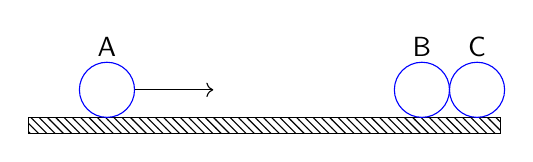
\begin{tikzpicture}
\draw[pattern=north west lines](0,-0.2) rectangle (6,0);
\foreach \x/\y in {1/A,5/B,5.7/C}{
\node at(\x,0.35) [circle,draw, blue, minimum size=0.7cm]{ };
\node at (\x,0.9){\y};}
\draw [->](1.35,0.35)--(2.35,0.35);

\end{tikzpicture}\\

A, B dan C adalah tiga buah bola biliar yang terletak di atas suatu permukaan yang licin. Bola B dan C bersentuhan. Jika bola A dipukul dan bergerak menumbuk bola b maka sesaat setelah tumbukan akan didapati . . . 
\pilgan{
\item A berhenti dan B terus bergerak
\item A terpantul balik, B berhenti, dan C bergerak
\item [\lingkaran{C.}]A dan B berhenti, C terus bergerak
\item A, B , dan C terus bergerak
\item A terpantul balik, B dan C terus bergerak
} 

\hide{
dengan anggapan massa sama dan lenting sempurna, maka saat A dengan kecepatan $v$ mengenai B
\begin{align*}
\Sigma p_A &=\Sigma p_B\\
\coret{m_A}.v_A+\coret{m_B}.v_B&=\coret{m_A}.v_A'+\coret{m_B}.v_B'\\
v_A+v_B &=v_A'+v_B'\\
v_A+0 &=v_A'+v_B'\\
v_A &=v_A'+v_B'\\
v_A'+v_B' &=v_A \text{  (1) }
\end{align*}
Karena $e=1$
\begin{align*}
e&=1\\
1&=\frac{-(v_A'-v_B')}{(v_A-v_B)}\\
v_A-0&=v_B'-v_A'\\
-v_A'+v_B'&=v_A\text{  (2) }
\end{align*}
Hasil elimimasi (1) dan (2)\\
$2v_A'=0$ dan $ v_A'=0$\\
Artinya benda A lalu berhenti, sedangkan $v_B'=v_A=v$ \\
Saat B bergerak dengan kecepatan $v$ dan menggerakkan C, dilihat bahwa kasusnya sama "satu bergerak, satu berhenti, massa sama" maka B akan berhenti dan C bergerak dengan kecepatan $v$
}



\item Kecepatan peluru saat lepas dari larasnya 200 m/s. Bila massa peluru dan senapan masing-masing 10 g dan 5 kg, kecepatan dorong senapan terhadap bahu penembak saat peluru lepas dari larasnya adalah . . . 
\pilgan{
\item -0,1 m/s
\item -0,2 m/s
\item -0,3 m/s
\item [\lingkaran{D.}]-0,4 m/s
\item -0,5 m/s
}

\hide{
$m_p$=0,01kg $m_b$=5 kg\\
mula-mula peluru dan bahu diam, $v_p'$=200 m/s ditanya $v_b'$
\begin{align*}
\Sigma p_1 &= \Sigma p_2\\
m_p.v_p+m_b.v_b &=m_p.v_p'+m_b.v_b'\\
0&=0,01.200+5.v_b'\\
v_b'&=\frac{-2}{5}\\
v_b'&=-0,4 \text{m/s}
\end{align*}
}

\item Sebuah benda menumbuk balok yang diam di atas lantai dengan kecepatan 20 m/s. Setelah tumbukan, balok terpental dengan kecepatan 15 m/s searah kecepatan semula. Kecepatan benda setelah tumbukan bila besar koefisien restitusi $e=0,4$ adalah . . . 
\pilgan{ 
\item [\lingkaran{A.}]7 m/s searah dengan kecepatan semula
\item 7 m/s  berlawanan arah dengan kecepatan semula
\item 8 m/s searah dengan kecepatan semula
\item 8 m/s berlawanan dengan kecepatan semula
\item 10 m/s searah dengan kecepatan semula
}
\hide{
Diketahui $v_{benda}=v_A$\\
\phantom{Diketahui}$v_{balok}=v_B$\\
\phantom{Diketahui} $e=0,4$
\begin{align*}
e&=0,4\\
0,4&=\frac{-(v_A'-v_B')}{(v_A-v_B)}\\
0,4.v_A-0,4.v_B&=v_B'-v_A' \\
8-0&=15-v_A'\\
v_A'&=7 \text{m/s   searah} 
\end{align*}
}

\item Perahu bermassa 150 kg dan orang dalam perahu bermassa 50 kg bergerak dengan kecepatan 10 m/s, orang tersebut melompati perahu dengan kecepatan 5 m/s, berlawanan dengan arah gerak perahu. Kecepatan akhir perahu adalah . . . \\
\pilgan{
\item [\lingkaran{A.}]15 m/s
\item 10 m/s
\item 5 m/s
\item 20 m/s
\item 25m/s
}
\hide{
keadaan awal dan akhir tanpa ada gaya dari luar, maka berlaku kekekalan momentum. kecepatan orang 5 m/s berlawanan arah perahu 
\begin{align*}
\Sigma p &= \Sigma p'\\
(m_p+m_o)v&=m_p.v_p'+m_o.v_o'\\
(150+50).10&=150.v_p'+50.(-5)\\
2000+250&=150.v_p'\\
v_p'&=\frac{2250}{150}=15 \text { m/s}
\end{align*}

}
\item Peluru dengan massa 0,01 kg dan kecepatan 1000 m/s mengenai dan menembus sebuah balok dengan massa 100kg yang diam di atas bisang datar tanpa gesekan. Kecepatan peluru setelah menembus balok adalah 100 m/s. Kecepatan balok setelah tertembus peluru adalah . . . .\\
\pilgan{
\item 900 m/s
\item 90 m/s
\item 9 m/s
\item 0,9 m/s
\item [\lingkaran{E.}]0,09 m/s
} 
\hide{
$m_p$ = 0,01 kg  $v_p$ = 1000 m/s \\
$m_b$ = 100 kg  $v_b'$ = . . . ?
\begin{align*}
\Sigma p  &= \Sigma p'\\
m_p.v_p+m_b.v_b &= m_p.v_p'+m_b.v_b'\\
0,01.1000+100.0 &= 0,01.100 + m_b.v_b'\\
v_b'&= \frac{10-1}{100}=0,09 \text {m/s}
\end{align*}
}


\item Sebuah peluru bermassa 8 g ditembakkan ke dalam sebuah balok kayu bermassa 10 kg sehingga peluru menancap ke dalam balok. Dalam keadaan ini balok yang semula diam kemudian bergerak dengan kecepatan 50 cm/s. Berapakah kecepatan awal peluru?\\
\pilgan{
\item [\lingkaran{A.}]625,5 m/s
\item 625,0 m/s
\item 62,55 m/s
\item 62,50 m/s
\item 650 m/s
}
\hide{
$v_{bp}$ = 0,5 m/s , balok dan peluru bergabung\\
\begin{align*}
\Sigma p &= \Sigma p'\\
m_b.v_b+m_p.v_p &= (m_b+m+p).v_{bp}\\
10.0+0,008.v_p &= (10,008).0,5 \\
v_p &= \frac{5,004}{0,008}= 625,5 \text {m/s}
\end{align*}

}
\item Sebuah peluru bermassa 10 g ditembakkan ke dalam suatu ayunan balistik yang bermassa 1490 g dan peluru bersarang dalam balok. Pada saat ayunan mencapai tinggi maksimum, ternyata balok dan peluru naik setinggi 5 m. Kecepatan peluru mengenai balok adalah . . . .\\
\pilgan{
\item 500 m/s
\item 1000 m/s
\item [\lingkaran{C.}]1500 m/s
\item 2000 m/s
\item 2500 m/s
}
\hide{
saat naik sampai titik tertinggi berarti energi kinetik diubah menjadi energi potensial
\begin{align*}
\frac{1}{2}mv^2 &= m.g.h\\
\frac{1}{2}\coret{m_{bp}}.v^2 &=\coret{ m_{bp}}.g.h\\
v^2 &= 2.10.5 \\
v &= 10 \text {m/s}
\end{align*}}
\hide{
$v$ = 10 m/s adalah kecepatan balok bersama peluru. Maka berdasarkan kekekalan momentum \\
\begin{align*}
\Sigma p &= \Sigma p'\\
m_p.v_p+m_b.v_b &= (m_b+m_p)v'\\
0,01.v_p+1,49.0 &= (1,5).10\\
0,01.v_p&= \frac{15}{0,01}\\
v_p &= 1500 \text {m/s}
\end{align*}

}
\item Dua balok bermasa $m_1$ = 2 kg dan $m_2$ = 4 kg saling mendekati di atas bidang licin. Laju masing-masing adalah $v_1$ = 5 m/s dan $v_2$ = 10 m/s. Jika kedua balok saling bertumbukan, momentum linear . . . .
\pernyataan{
\item sistem adalah 30 kgm/s
\item balok kedua adalah 30 kgm/s jika laju balok pertama nol
\item balok kedua 20 kgm/s jika laju balok pertama 5 m/s ke kiri
\item balok pertama 30 kgm/s jika laju balok kedua adalah nol
}Pernyataan yang benar adalah . . . 
\pilgan{
\item 1,2, dan 3 
\item 1 dan 3 
\item 2 dan 4
\item 4 saja
\item [\lingkaran{E.}]1,2,3, dan 4
}
\hide{
\pernyataan{
\item sistem adalah 30 kgm/s \centang{ }	\\
$p=m_1.v_1+m_2.v_2$\\
$p= 2.5 + 4.(-10)= -30$\\
 \merah{\small{berarti besarnya momentum linear sistem adalah 30 kgms (arahnya searah dengan benda 2}}
\item balok kedua adalah 30 kgm/s jika laju balok pertama nol\centang{ }
\merah{\vspace{-0.5cm} \small{\begin{align*}
\Sigma p &= \Sigma p'\\
m_1.v_1+m_2.v_2&=m_1.v_1'+p_2'\\
2.5+4(-10)&=2.0+p_2'\\
p_2'&=-30 \text{kgm/s}
\end{align*}}} \vspace{-0.5cm}
\item balok kedua 20 kgm/s jika laju balok pertama 5 m/s ke kiri \centang{ }
\merah{\vspace{-0.5cm} \small{\begin{align*}
\Sigma p &= \Sigma p'\\
m_1.v_1+m_2.v_2&=m_1.v_1'+p_2'\\
2.5+4(-10)&=2.(-5)+p_2'\\
p_2'&=-20 \text{kgm/s}
\end{align*}}} \vspace{-0.5cm}}}
\hide {
\pernyataan{
\setcounter{enumii}{2}
\item balok pertama 30 kgm/s jika laju balok kedua adalah nol \centang { }
\merah{ \small{\begin{align*}
\Sigma p &= \Sigma p'\\
m_1.v_1+m_2.v_2&=m_1.v_1'+p_2'\\
2.5+4(-10)&=p_1+4.0\\
p_1'&=-30 \text{kgm/s}
\end{align*}}} \vspace{-0.5cm}
}}

\item Balok bermassa 1 kg digantung pada seutas tali sepanjang 5 m, ditembak oleh peluru bermassa 10 g. Ternyata, peluru bersarang di dalam balok dan terjadi putaran satu kali lingkaran penuh. Kecepatan minimal peluru adalah . . . \\
\pilgan{
\item 305 m/s
\item 355 m/s
\item 405 m/s
\item 455 m/s
\item [\lingkaran{E.}]505 m/s
}
\hide{
Untuk melakukan satu putaran penuh diperlukan kecepatan awal tertentu. Digunakan konsep GMB dan kekekalan energi\\
Pada ketinggan maksimal lingkaran vertikal,kecepatan minimal agar timbul satu putaran adalah saat tegangan tali = 0
\begin{align*}
\Sigma F_s &= mg + N \\
\Sigma F_s &=mg + 0 \\
\coret{m} .\frac{v^2}{r} &= \coret{m}g\\
v^2 &= g.r
\end{align*}

Lalu menurut hukum kekekalan energi
\begin{align*}
EM &= EM'\\
EP + EK &= EP_2  + EK_2 \\
0 + \frac{1}{2}\coret{m}v_1^2 &= \coret{m}gh + \frac{1}{2}\coret{m}v^2\\
\frac{1}{2}v^2&=10.(2.50)+\frac{1}{2}gR\\
v^2&=2500 \\
v&=50 \text{ m/s}
\end{align*}
kecepatan $v$ tersebut adalah kecepatan balok dan peluru. Untuk menentukan kecepatan peluru sebelum bersarang pada balok, gunakan kekekalan momentum
\begin{align*}
\Sigma p &= \Sigma p'\\
m_p.v_p+m_b.v_b&=(m_p+m_b)v'\\
0,01.v_p & = (1,01).50\\
v_p&= 5050 \text {m/s}
\end{align*}
} \hide {
Jadi kecepatan peluru adalah 5050 m/s. Namun di pilihan tidak ada, mungkin karena nilai panjang tali yang 50m. 
}

\item Bila dua buah benda bertumbukan secara tidak lenting sempurna, maka pernyataan di bawah ini benar, kecuali . . .
\pilgan{
\item setelah tumbukan kecepatan kedua benda itu sama besar
\item kecepatan kedua benda sebelum dan sesudah tumbukan tidak sama besar
\item jumlah momentum kedua benda sebelum dan sesudh tumbukan sama besar
\item koefisien restitusinya nol
\item [\lingkaran{E.}] sebelum dan sesudah tumbukan jumlah energi kinetik kedua benda itu sama besar
}
\hide{
Pada pernyataan A, kecepatan kedua benda sama besar bisa terjadi jika kedua benda bergabung \\ 
}
\hide{
Pada pernyataan B, kecepatan akan sama besar tidak dapat ditentukan. Namun ada kemungkinan untuk sama besar \\ 

Pada pernyataan C, jumlah momentum sama besar adalah hal yang pasti. Karena tanpa ada yang gaya luar yang bekerja maka momentum kekal \\
Pada pernyataan D, tidak lenting sempurna mencakup tidak lenting sama sekali, dan tidak lenting sama sekali koefisien restitusinya adalah nol.\\
Pada pernyatan E \silang {  }, salah satu sifat lenting tidak sempurna adalah jumlah energi kinetiknya \merah{tidak kekal}. Karena sebagian energi diubah menjadi energi suara, panas, dsb
}

\item Dua benda masing-masing massanya 2 kg dan 3 kg, bergerak berlawanan arah, dengan kecepatan 4 m/s dan 6 m/s. Jika setelah tumbukan kedua benda tersebut bersatu, tentukanlah besarnya energi yang hilang pada saat terjadi tumbukan!
\pilgan{
\item 1,2 J
\item 2,4 J
\item 3,6 J
\item 4,2 J
\item 5,6 J
\item [\lingkaran{F.}] 60 J
}
\hide{
Sebelum bertumbukan energi kinetik total adalah 
\begin{align*}
\frac{1}{2}m_1.v_1^2 + \frac{1}{2}m_2.v_2^2 & = \frac{1}{2}2.4^2 + \frac{1}{2}3.6^2\\
EK_1 & = 16 + 54 = 70 \text{ J}
\end{align*}
Menghitung kecepatan gerak bersama dengan kekekalan momentum 
\begin{align*}
\Sigma p &= \Sigma p'\\
m_1.v_1+m_2.v_2&=(m_1+m_2)v'\\
2.4+3.(-6) &= (5).v'\\
v'&= \frac{-10}{5}=-2\text {m/s}
\end{align*}
Selisih EK 
\begin{align*}
\Delta EK &= EK_1 - EK_2\\
\Delta EK & = 70 -\frac{1}{2}m_{total}.v'^2\\
\Delta EK & = 70 - 10 =60 \text{J}
\end{align*}
}
\item Diketahui benda A dengan laju 8 m/s dan benda B dengan laju 4 m/s mengalami tumbukan. Bila koefisien restitusi, $e = \frac{1}{3}$. Tentukan perubahan energi kinetik sebelum dan sesudah tumbuhan!
\pilgan{
\item 100 J
\item 105 J
\item 112 J
\item [\lingkaran{D.}]120 J
\item 244 J
}
\hide{
\begin{align*}
e &= \frac {-(v_2'-v_1')}{(v_2-v_1)}\\
\frac{1}{3} &= \frac{-(v_2'-v_1')}{(-4-8)}\\
\frac{-12}{3} &= v_1' - v_2' \\
v_1' -v_2' &= -4 \text {   persm (1)}
\end{align*}
Dengan persamaan kekekalan momentum 
\begin{align*}
\Sigma p &= \Sigma p'\\
m_1.v_1+m_2.v_2&=m_1.v_1'+m_2.v_2'\\
5.8+3.(-4) & =5.v_1' + 3.v_2'\\
5v_1'+3v_2'&=28 \text {    persm (2)}
\end{align*}
Eliminasi persamaan 1 dan 2 maka diperoleh\\
$v_1'$ = 2 m/s   dan $v_2'$ = 6 m/s \\
Selisih Ek sebelum dan sesudah
\small{\begin{align*}
\Delta EK &= EK_2 - EK_1\\
\Delta EK &= (\frac{1}{2}m.v_1'^2+\frac{1}{2}mv_2'^2)- (\frac{1}{2}m.v_1^2+\frac{1}{2}mv_2^2)\\
\Delta Ek &= \frac{1}{2}(m_2.(v_2'^2-v_2^2)+m_1.(v_1'^2-v_1')\\
\Delta Ek &= -120 \text{ J}
\end{align*} 
}
}


\item Sebuah bola dijatuhkan di atas lantai, tepat sebelum mengenai lantai energi kinetiknya = E. Tepat saat terpantul, energi kiinetik menjadi $\frac{1}{4}$E. Koefisien restitusi benda dengan lantai adalah . . .
\pilgan{
\item 0,6
\item [\lingkaran{B.}]0,5 
\item 0,4
\item 0,2
\item 0,1
}
\hide{
Pada soal ini kita tentukan bahwa kecepatan lantai adalah $v_2$ dan lantai adalah $v_1$. Lantai tetap pada posisinya, tidak bergerak. Maka gunakan persamaan resitusi
\begin{align*}
e &= \frac{-(v_2'-v_1')}{(v_2-v_1)} \\
e &= \frac{-(v_2'-0)}{(v_2-0)}\\
\end{align*}
Padahal $E=\frac{1}{2}mv^2$ maka $v=\sqrt{\frac{2E}{m}}$
\begin {align*}
e &= \frac {\sqrt{\frac{2(\frac{1}{4}E)}{m}}}  {\sqrt{\frac{2(E)}{m}}}\\
e &=\sqrt {\frac{1}{4}}\\
e &= \frac{1}{2} = 0,5 
\end{align*}
}

\item Sebuah bola tenis yang massanya 100 g dilepaskan dari ketingian tertentu. Pada pemantulan pertama tinggi yang dapat dicapai adalah 3,0 m dan pada pemantulan kedua dalah 1,5 m. Tinggi bola tenis mula-mula adalah . . . .
\pilgan{
\item 2 m
\item 4 m
\item [\lingkaran{C.}]6 m
\item 8 m
\item 9 m
}
\hide{
Karena benda yang berinteraksi tetap, yakni bola tenis dan lantai, maka koefisien restitusinya tetap. Jika $h_1$ adalah tinggi mula-mula, $h_2$ tinggi pantulan pertama, $h_3$ adalah tinggi pantulan kedua
\begin{align*}
e&=\sqrt{\frac{h_2}{h_1}}\\
e&=\sqrt{\frac{h_3}{h_2}}\\
\sqrt{\frac{h_2}{h_1}} &= \sqrt{\frac{h_3}{h_2}}\\
\frac{h_2}{h_1}&=\frac{h_3}{h_2}\\
h_1&=\frac{3.3}{1,5}=6 \text{ m}
\end{align*}}


\item Sebuah bola dijatuhkan dari ketinggian 5 m dan terpental hingga mencapai ketinggian 0,8 m. Koefisien restitusi antara lantai dan bola itu adalah sebesar . . . 
\pilgan{
\item 0,3
\item [\lingkaran{B.}]0,4
\item 0,5
\item 0,6
\item 0,7
}
\hide{
\begin{align*}
e&=\sqrt{\frac{h_2}{h_1}}\\
e&=\sqrt{\frac{0,8}{5}}\\
e&= 0,4
\end{align*}

}
\item Bola yang massanya 200 g dijatuhkan dari ketinggian 5 m di atas lantai mendatar. Jika koefisien tumbukan antara bola dan lantai 0,5, ketinggian bola setelah memantul dari lantai adalah. . . .
\pilgan{
\item 3,50 m
\item 2,50 m
\item 2,0 m
\item 1,50 m
\item [\lingkaran{E.}]1,25 m
}
\hide{
\begin{align*}
e&=\sqrt{\frac{h_2}{h_1}}\\
0,5&=\sqrt{\frac{h_2}{5}}\\
0,25&=\frac{h_2}{5}\\
h_2 &=1,25 \text { m} 
\end{align*}

}
\item Agar sebuah pesawat antariksa dapat mencapai orbit, maka pesawat itu harus memperoleh kelajuan sangat tinggi kira-kira 8000 m/s. Anggap massa pesawat itu 10.000 kg. Kelajuan tertinggi semburan gas keluar dari roket kira-kira 4000 m/s. (setengah dari kelajuan yang harus dicapai pesawat). Hitung massa bahan bakar yang diperlukan oleh roket untuk meluncurkan pesawat antariksa menuju orbitnya!
\pilgan{ 
\item [\lingkaran{A.}]20.000 kg
\item 2000 kg
\item 10.000 kg
\item 1.000 kg
\item 25.000 kg
}
\hide{
Dengan asumsi bahwa pesawat dan bahan bakar adalah dua benda yang jadi satu. Saat bahan bakar keluar, pesawat bergerak ke depan. Keadaan seperti ini diselesaikan dengan menggunakan konsep kekekalan momentum.\\
$v_r$ awal = 0\\
$v_b$ awal =0 \\
$v_r'$ = -4000 m/s \\
$v_r'$ = 8.000 kg \\
Ditanya $m_r$ =. . . ?
\begin{align*}
m_r.v_r+m_b.v_b&=m_r.v_r' + m_b.v_b'\\
\end{align*}
\begin{align*}0 &=10000.8000 + m_b.(-4000)\\
m_b &= 20.000 \text { kg}
\end{align*}

}
\item Sebuah roket berdiri di atas pelataran. Setelah mesinnya dihidupkan, gas yang disemburkan oleh roket sebanyak 1.500 kg/s. Kecepatan molekul gas 50 km/s. Jika semburan gas itu ternyata cukup untuk mengangkatnya perlahan-lahan meninggalkan landasannya, massa roket mula-mula adalah . . .(g = 10 m/s$^2$)
\pilgan {\item [\lingkaran{A.}] $7,5 \times 10^6$ kg
\item $7,0 \times 10^6$ kg
\item $6,5 \times 10^6$ kg
\item $6,0 \times 10^6$ kg
\item  $5,5 \times 10^6$ kg
}
\hide {
Diketahui $\Delta m/\Delta t $ = 1500 kg/s\\
$v$ = 50000 m/s \\
Agar bisa mengangkat perlahan-lahan berarti percepatan $a$ roket tidak nol (0)\\
\begin{align*}
F.\Delta t &= \Delta p\\
F &= \frac{\Delta p}{\Delta t}\\
F &= \frac{\Delta m .v}{\Delta t}\\
F &= \frac{\Delta m}{\Delta t}v\\
F &= 1500.50000 = 7,5 \times 10^7
\end{align*}
Untuk menentukan massa benda kita gunakan bahwa berat adalah gaya, maka :
\begin{align*}
F &=m.g \\
m &= \frac{F}{g} = 7,5 \times 10^6
\end{align*}
}

\item Sebuah roket bermassa 200 ton diarahkan tegak lurus ke atas. Jika mesin roket mengeluarkan/membakar bahan bakar sebanyak 20 kg tiap skeon, berapakah kecepatan molekul gas yang terbakar itu . . ..  (pengurangan massa roket karena pembakaran bahan bakar sedikit sehingga boleh diabaikan)
\pilgan{
\item 60 km/s
\item 70 km/s
\item 80 km/s
\item 90 km/s
\item [\lingkaran{E.}] 100 km/s
}
\hide{
massa roket adalah 200 ton, berarti beratnya roket adalah 2.000.000 N
\begin{align*}
F.\Delta t &= \Delta p\\
F &= \frac{\Delta p}{\Delta t}\\
F &= \frac{\Delta m .v}{\Delta t}\\
F &= \frac{\Delta m}{\Delta t}v\\
2 \times 10^6 &= 20.v \\
v &= 1 \times 10^5 = 100 \text{ km/s}
\end{align*}
}
\item Peristiwa yang memenuhi hukum kekekalan momentum, hukum kekekalan energi kinetik, dan memiliki koefisien restitusi $e=1$ adalah jenis tumbukan . . . . .
\pilgan{
\item tidak lenting
\item tidak lenting sama sekali
\item lenting sebagian
\item [\lingkaran{D.}]lenting sempurna
\item lenting
}

\item Sebuah benda yang mempunyai massa 50 gram bergerak lurus dengan kecepatan 30 m/s. Akibat pengaruh gaya gesek benda mengalami perlambatan 2 m/s$^2$. Besar momentum benda setelah bergerak 5 detik adalah . . . 
\pilgan{
\item 10 kg m/s
\item 12,5 kg m/s
\item 15 kg m/s
\item [\lingkaran{D.}]20 kg m/s
\item 22,5 kg m/s
}
\hide{
Gaya gesek benda adalah 2 m/s$^2$ dan waktu perlambatan adalah 5 detik. Menurut persamaan impuls-momentum maka 
\begin{align*}
I &= F. \Delta t \\
\Delta p &= F. \Delta t \\
m. \Delta v &= F. \Delta t \\
\coret{m} . (v_2 -v_1) &= \coret{m}a.\Delta t \\
(v_2 - 30) &= 2.5\\
v_2 &= 40 \text { m/s}
\end{align*}
Jadi besar momenum benda setelah bergerak adalah . . . 
\begin{align*}
p &= m.v_2\\
p&= 0,5 .40 = 20 \text {kg m/s}
\end{align*}}

\item Sebuah bola kasti yang masanya 0,1 kg dilembar horisontal ke kanan dengan kecepatan 20 m/s, kemudian dipukul dengan impuls gaya 6 Ns berlawanan dengan arah gerak semula. Jika kontak antara bola dan pemukul 0,1 ms, maka kecepatan akhir bola adalah . . . .
\pilgan{
\item 10 m/s ke kiri
\item 20 m/s ke kanan
\item 25 m/s ke kiri 
\item 35 m/s ke kanan
\item [\lingkaran{E.}]40 m/s ke kiri
}
\hide{ 
Kecepatan bola kasti awal adalah $v_1$ = 20 m/s dan impulsnya adalah -6Ns 
\begin{align*} 
I &= \Delta p \\
I &= m .\Delta p \\
I &= 0,1.(v_2-v_1) \\
-6 &= 0,1 (v_2 -20)\\
v_2 &= -40 \text { m/s}
\end{align*}
Jadi kecepatan akhir bola adalah 4 m/s ke arah kiri (tanda negatif berlawanan arah dengan gerak benda mula-mula)
}


\item Dari ketinggian tertentu suatu bola tenis dengan massa 200 gram dijatuhkan tanpa kecepatan awal. Jika setelah pemantulan pertama tinggi yang dicapai 4 m dan pemantulan kedua 2 m, maka tinggi bola mula-mula adalah . . . .
\pilgan{
\item 12 m
\item 10 m
\item [\lingkaran{C.}]8 m
\item 6 m
\item 5 m
}
\hide{
\begin{align*}
e &= \sqrt{\frac{h_2}{h_1}}\\
e &= \sqrt{\frac{h_3}{h_2}}\\
\sqrt{\frac{h_2}{h_1}} &= \sqrt {\frac{h_3}{h_2}}\\
h_1&=\frac{h_2.h_2}{h_3}=\frac{16}{2} = 8\text{m}
\end{align*}
}

\item Seorang yang massanya 60 kg berdiri pada papan yang massanya 10 kg yang diam di lantai yang licin. Jika tiba-tiba orang tadi meloncat dengan kecepatan 20 m/s, maka papan melesat dengan kecepatan . . . 
\pilgan{
\item  20 m/s
\item  40 m/s
\item  60 m/s
\item  100 m/s
\item  [\lingkaran{E.}]120 m/s
}
\hide{
misalnya massa orang adalah $m_o$=60 kg dan massa papan $m_p$=10 kg. Kedua benda diam, berarti momentum awal $p=0$
\begin{align*}
\Sigma p &= \Sigma p' \\
0 &= m_o.v_o' + m_p.v_p'\\
0&= 60.20 + 10.v_p'\\
v_p' &= 120 \text {  m/s}
\end{align*}

}

\item Sebuah bola bergerak dengan kecepatan 10 m/s horisontal  ke barat. Jika massa bola 400 gram dan dipukul horisontal ke timur dengan gaya 40 N, maka waktu yang diperlukan untuk menghentikan adalah . . . 
\pilgan{
\item 0,20 sekon
\item 0,25 sekon
\item 0,10 sekon
\item 0,30 sekon
\item 0,50 sekon
}
\hide{
\begin{tikzpicture}
\draw

\end{tikzpicture}


}

\end{enumerate}    

\end{multicols*}
 \vspace{1cm}
%-------------------------------------------




 \end{document}
